\documentclass{standalone}
\usepackage{tikz}
\begin{document}
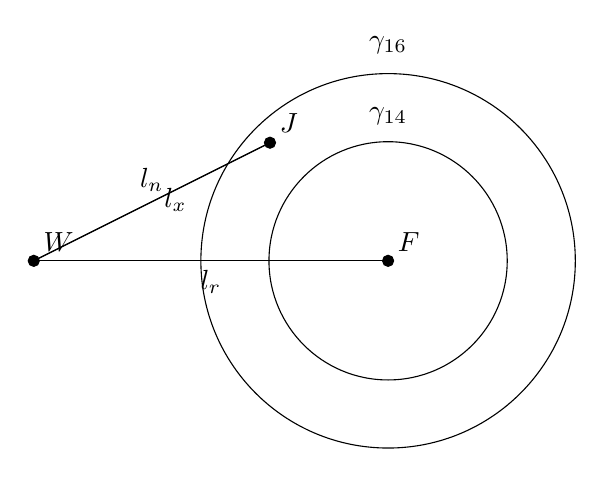
\begin{tikzpicture}[scale=1.0]
  \filldraw (0.0, 0.0) circle (2pt) node[above right] {$W$};
  \filldraw (3.0, 1.5) circle (2pt) node[above right] {$J$};
  \filldraw (4.5, 0.0) circle (2pt) node[above right] {$F$};
  \draw (0.0, 0.0) -- (4.5, 0.0) node[midway, below] {$l_r$};
  \draw (0.0, 0.0) -- (3.0, 1.5) node[midway, above] {$l_n$};
  \draw (0.0, 0.0) -- (3.0, 1.5) node[midway, below, shift={(0.3,0.3)}] {$l_x$};
  \draw (4.5, 0.0) circle (1.5129) node[above=1.6cm] {$\gamma_{14}$};
  \draw (4.5, 0.0) circle (2.3777) node[above=2.5cm] {$\gamma_{16}$};
\end{tikzpicture}
\end{document}